\ylDisplay{Lääts ja selle fookus} % Ülesande nimi
{Koit Timpmann} % Autor
{lõppvoor} % Voor
{2018} % Aasta
{P 5} % Ülesande nr.
{3} % Raskustase
{
% Teema: Valgusõpetus
\ifStatement
Joonisel on kujutatud valguspunkt, sellest läätse abil saadud kujutis ning läätse optiline peatelg $O_1$$O_2$. Konstrueerige läätse ja selle fookuse asukohad kõikide võimalike juhtude jaoks. Esitage lahendus lisalehel.
\begin{center}
	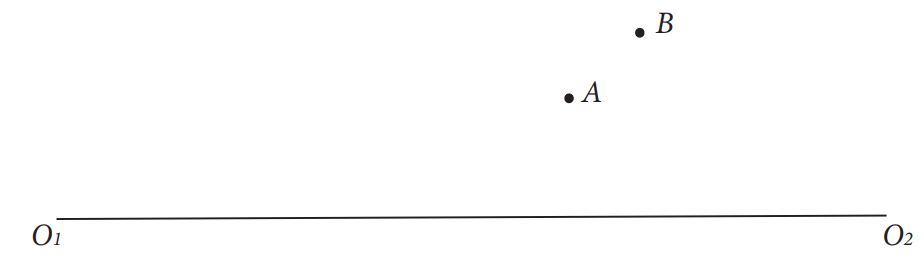
\includegraphics[width=0.5\linewidth]{2018-v3p-05-yl.PNG}
\end{center}
\fi
\ifHint
Lahendus võib olla saadud nii kumera kui ka nõgusaläätsega.
\fi
\ifSolution
Kui A on valguspunkt ja B selle kujutis, siis on tegemist kumerläätsega, mis töötab nagu luup.
\begin{center}
	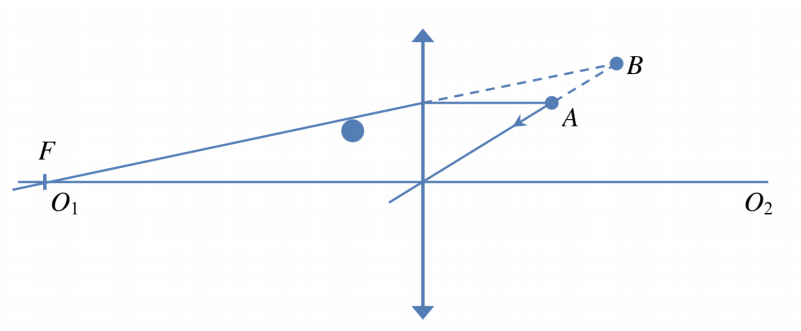
\includegraphics[width=0.5\linewidth]{2018-v3p-05-lah1.PNG}
\end{center}
Kui A on valguspunkti kujutis ja B valguspunkt, siis on tegemist nõgusläätsega.
\begin{center}
	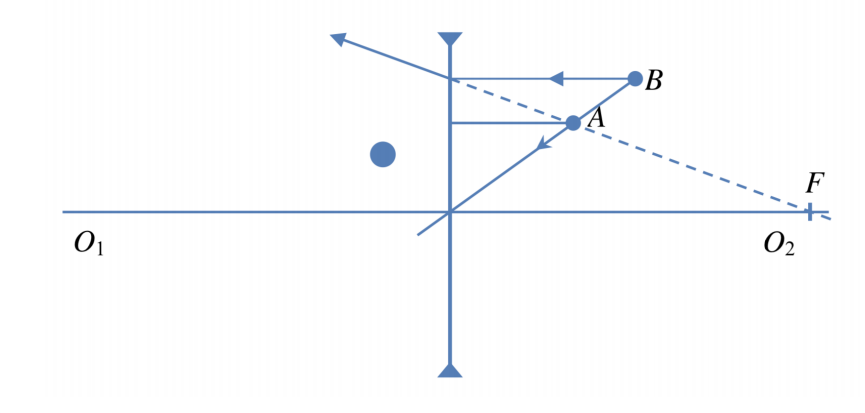
\includegraphics[width=0.5\linewidth]{2018-v3p-05-lah2.PNG}
\end{center}
\fi
}